\chapter{USB}
USB ist eine Schnittstelle, welche so gut wie alle modernen Rechner besitzen. Es ist unter anderem Möglich darüber Geräte wie Kopfhörer, Joysticks aber auch Wechseldatenträger an zu schließen. Im letzteren Bereich ersetzt USB die bisher vorherrschende CD/DVD-Technologie, da auf einem USB Stick mehr Daten in höherer Geschwindigkeit gespeichert werden können und diese zudem handlicher sind. Jedoch birgt die USB-Technologie auch Gefahren, welche in den folgenden Sektionen beschrieben werden. Anschließend werden in \ref{Deskriptoren} die Deskriptoren beschrieben, welche eine USB-Gerät mit sich bringt und welche bei der geprüften Policie zur Prüfung verwendet wurden.

\section{Gefahren bei USB}\label{GefBeiUSB}
USB-Geräte stellen Gefahren auf verschiedenen Ebenen dar. Zum einen werden USB-Sticks, zumindest in dem Szenario, das hier betrachtet wurde, von Dritten an Mitarbeiter gegeben. Das bedeutet, dass der Dritte, insofern dieser die nötige kriminelle Energie aufweist, ein präpariertes Gerät einschicken könnte. Erschwerend kommt hinzu, dass der Mitarbeiter keine Möglichkeit hat, ein böses USB-Gerät von einem normalen zu unterscheiden. Auch besteht die Möglichkeit für den Dritten den Angriff über längere Zeit vorzubereiten, da kein Zeitdruck besteht. Im Gegenteil, USB-Geräte sind gerade noch im Aufwärtstrend und werden sich wohl langfristig auf dem Markt etablieren. TODO CD vs USB Statistik. Im folgenden werden einige der Risiken dargestellt

\subsection{Viren}
Viren sind eine wachsende Bedrohung in der heutigen Zeit. Vor einigen Jahren waren einige wenige Virenfamilien weit verbreitet. So konnten Virenschutzhersteller über signaturbasierte Suchalgorithmen nach bekannten Mustern suchen und Viren identifizieren. In den letzten Jahren zeichnet sich jedoch der Trend ab, dass Viren sich schneller weiterentwickeln und zudem oft polymorph programmiert sind, also ihr aussehen bei einer Infektion verändern. Dadurch werden signaturbasierte Erkennungen immer ineffizienter und die Gefahr, dass ein Rechner unerkannt Infiziert wird, steigt. Eine Infektion passiert zumeist über sogenannte Browserexploits, also präparierte Webseiten, welche Lücken in der Software des Users nutzten, oder Anhänge an Spammails. In dem von uns betrachteten Szenario würde ein krimineller Dritter oder aber auch ein unwissender Dritter, dessen Rechner im Vorfeld von einem Virus infiziert wurde, einen USB-Stick mit einem Virus einschicken. Ein Beispiel für einen solchen Virus wäre ein Trojaner. Dies sind Programm, welches sich als normale Software tarnt aber Schadcodefunktionalität mitliefert. \cite{Stamp2006} Will ein Benutzer das vermeidlich sinnvolle Programm installieren, wird im Hintergrund unbemerkt die Schadroutine mit installiert und gestartet. Dieser Schadecode hat oftmals Funktionalitäten wie Keylogger, Backdoors oder ein Rootkit. Als Beispiel könnte man hier den in \textit{Metasploit}\footnote{http://www.metasploit.com/} enthaltenen \textit{Meterpreter} nennen, dessen Funktionen jedoch weit über die oben genannten hinaus gehen \footnote{http://www.offensive-security.com/metasploit-unleashed/Meterpreter\_Basics}. Hier muss also ein Benutzer also einen USB-Stick einstecken und ein darauf befindliches Programm starten, damit sich der Virus installieren kann. Ist dieser bereits bekannt, könnte ein auf dem System installierter Virenscanner diesen finden und bestenfalls blockieren. Jedoch ist es Aufgrund des Fortschritts immer öfter der Fall, dass Viren sich trotz gleicher Funktionalität ihr aussehen verändern und dadurch von den Pattern des Virenschutzes nicht mehr erfasst werden.
			
\subsection{Datenabfluss}
Neben den Gefahren von außen müssen jedoch auch sogenannte \glqq Inside-Threaths\grqq beachtet werden. Dies wären Mitarbeiter, welche z.B. interne IT-Systeme manipulieren, um sich Vorteile oder Reichtümer zu verschaffen. Bezogen auf USB wäre ein Risiko der Abfluss von vertraulichen oder wertvollen Daten, also wenn ein Mitarbeiter diese auf einem USB-Stick speichert und aus den Machtbereich des Unternehmens bringt. Anschließend könnte er diese Verkaufen oder sich zu bereichern, falls diese Daten zum Beispiel Bankdaten umfassten. Andere denkbar Beispiel wären Kundendaten, bei Benutzerkontos, Geschäftsberichte oder sonstige Unternehmensgeheimnisse. Diese können oft für Geld in einschlägigen Bereichen des Internets verkauft oder bei Geschäftsberichten zur Manipulation am Finanzmarkt genutzt werden. Auch wäre eine Abwerbung eines Mitarbeiters von einem anderen Unternehmen für Industriespionage denkbar.
Eine neue Bedrohung sind Geheimdienste, welche Personen in eine Unternehmen einschleusen oder Mitarbeiter abwerben, um Daten übe die Kunden zu sammeln. Dies wurde erst letztens durch von Edward Snowden veröffentlichte Dokumente publik.\footnote{https://firstlook.org/theintercept/2014/10/10/core-secrets/}



\subsection{Exploits auf Treiberebene}
Für den Mitarbeiter noch schwieriger zu entdecken sind Exploits auf Treiberebene. Dieses Vorgehen ist relativ neu, es wird dabei versucht Lücken im Treiber des Geräts auszunutzen. Hierzu muss ein Benutzer einen z.B. manipulierten USB-Stick nur einstecken. Es bedarf im Gegensatz zu normalen Viren keiner weiteren Interaktion des Users, da sich der Computer automatisch mit dem USB-Device kommuniziert um die Funktionen des Geräts zu erfahren und eventuell benötigte Treiber zu installieren. Hier beginnt das Gerät jedoch bereits bestimmte schädliche Zeichenfolgen an den  Computer zu senden, welche vom Treiber interpretiert und unter Umständen einen Buffer Overflow triggern können\footnote{https://srlabs.de/badusb/}. Durch diese Lücken kann dann auf dem Rechner des Benutzers Schadcode ausgeführt werden, ohne das dieser dies Bemerkt.


\section{Technische Ablauf beim Einstecken eines USB-Devices}
Dieser kurze Abschnitt gibt eine genauere, jedoch immer noch Oberfläche gehaltene Beschreibung der Schritte 2., 6. und 7. der Grafik \ref{fig:Ablauf}. Wird ein USB-Gerät eingesteckt, bekommt dieser über den USB-Anschluss Strom und sendet ein Ankündigungspaket. Der Computer reagiert darauf und fordert Informationen, also die in \ref{Deskriptoren} beschriebenen Felder, an. Das USB-Gerät überträgt diese an den PC. TODO Quelle

\section{Descriptoren}\label{descriptoren}
Der USB-Spezifikation, welche von dem USB Implementers Forum, Inc.\footnote{http://www.usb.org/about} festgelegt wird, sieht Felder vor, welche Informationen zu dem Gerät beinhalten.
\begin{wrapfigure}{l}{0pt}%{0.5\textwidth}
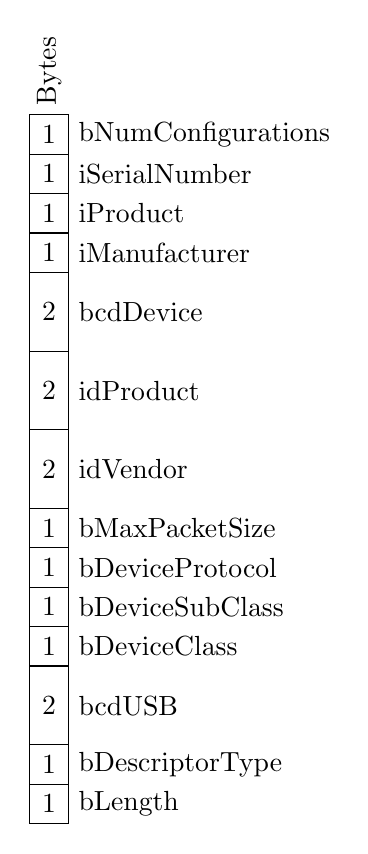
\begin{tikzpicture}[scale=1]
	\draw (0,0) rectangle (0.5,0.5);
	\draw (0.25, 0.25) node {1};
	\draw (0.5, 0.25) node[right]{bLength};
	
	\draw (0,0.5) rectangle (0.5,0.5);
	\draw (0.25, 0.75) node {1};
	\draw (0.5, 0.75) node[right]{bDescriptorType};
	
	\draw (0,1) rectangle (0.5,1);
	\draw (0.25,1.5) node {2};
	\draw (0.5,1.5) node[right]{bcdUSB};
	
	\draw (0,2) rectangle (0.5,0.5);
	\draw (0.25,2.25) node {1};
	\draw (0.5,2.25) node[right]{bDeviceClass};

	\draw (0,2.5) rectangle (0.5,0.5);
	\draw (0.25,2.75) node {1};
	\draw (0.5,2.75) node[right]{bDeviceSubClass};

	\draw (0,3) rectangle (0.5,0.5);
	\draw (0.25,3.25) node {1};
	\draw (0.5,3.25) node[right]{bDeviceProtocol};

	\draw (0,3.5) rectangle (0.5,0.5);
	\draw (0.25,3.75) node {1};
	\draw (0.5,3.75) node[right]{bMaxPacketSize};
	
	\draw (0,4) rectangle (0.5,1);
	\draw (0.25,4.5) node {2};
	\draw (0.5,4.5) node[right]{idVendor};
	
	\draw (0,5) rectangle (0.5,1);
	\draw (0.25,5.5) node {2};
	\draw (0.5,5.5) node[right]{idProduct};
	
	\draw (0,6) rectangle (0.5,1);
	\draw (0.25,6.5) node {2};
	\draw (0.5,6.5) node[right]{bcdDevice};
	
	\draw (0,7) rectangle (0.5,0.5);
	\draw (0.25,7.25) node {1};
	\draw (0.5,7.25) node[right]{iManufacturer};
	
	\draw (0,7.5) rectangle (0.5,0.5);
	\draw (0.25,7.75) node {1};
	\draw (0.5,7.75) node[right]{iProduct};
	
	\draw (0,8) rectangle (0.5,0.5);
	\draw (0.25,8.25) node {1};
	\draw (0.5,8.25) node[right]{iSerialNumber};
	
	
	\draw (0,8.5) rectangle (0.5,0.5);
	\draw (0.25,8.75) node {1};
	\draw (0.5,8.75) node[right]{bNumConfigurations};
	
	\draw (0,9) rectangle (0.5,0.5);
	
	\draw (0.25, 9) node[rotate=90, right] {Bytes};
\end{tikzpicture}
\caption{USB-Felder}
\end{wrapfigure}

Dies Umfasst die technische Informationen wie die Länge der gesamten Felder im \glqq bLength\grqq-Feld oder das Protokoll des Geräts im \glqq bDeviceProtocoll\grqq-Feld über Informationen für das Betriebssystem wie \glqq idVendor\grqq, \glqq idProduct\grqq, \glqq bDeviceSubClass\grqq und \glqq bDeviceClass\grqq. Diese Felder mit der jeweiligen Länge sind in der Grafik dargestellt. Ein Feld hat dabei zwischen ein und zwei Bytes. Die Felder \glqq bDeviceClass\grqq, \glqq bDeviceSubClass\grqq, \glqq bDeviceProtocol\grqq sowie \glqq idVendor\grqq werden vom Hersteller befüllt.\footnote{http://www.beyondlogic.org/usbnutshell/usb5.shtml} Das Betriebssystem nutzt die Felder meist um Treiber zu suchen oder auch das angeschlossene USB-Gerät gegen die Policie-Einstellungen zu prüfen. Um eigene Werte bei \textit{idProduct} oder \textit{idVendor}-Felder zu nutzten und damit sicher gestellt ist, dass nicht mehrere Hersteller die selbe \textit{idProduct} verwenden, müssen die Adressbereiche der \textit{idProduct} bei dem USB Implementers Forum, Inc. gekauft werden. Dazu gibt es zwei Möglichkeiten. Man kann entweder ein Mitglied werden, wobei kosten von 5000 USD jährlich anfallen oder einmalig 5000 USD für einen Adressraum zahlen, man darf dann jedoch nicht das offizielle USB-Logo verwenden. \footnote{http://www.usb.org/developers/vendor/} Im folgenden werden die für dieses Dokument interessanten Felder weiter erläutert:

%\begin{figure}[h]
%	\setlength{\unitlength}{0.14in} % selecting unit length
%	\centering % used for centering Figure
%	\begin{picture}(36,10) % picture environment with the size (dimensions)
%% 32 length units wide, and 15 units high.
%		\put(0,4){BlaBLab}
%		\put(0,0){\framebox(2,3){1}}
%		\put(2,0){\framebox(2,3){1}}
%		\put(4,0){\framebox(4,3){1}}
%		\put(8,0){\framebox(2,3){1}}
%		\put(10,0){\framebox(2,3){1}}
%		\put(12,0){\framebox(2,3){1}}
%		\put(14,0){\framebox(2,3){1}}
%		\put(16,0){\framebox(4,3){1}}
%		\put(20,0){\framebox(4,3){1}}
%		\put(24,0){\framebox(4,3){1}}
%		\put(28,0){\framebox(2,3){1}}
%		\put(30,0){\framebox(2,3){1}}
%		\put(32,0){\framebox(2,3){1}}
%		\put(34,0){\framebox(2,3){1}}
%		\put(23,4){\framebox(6,3){$H_{C}(q)$}}
%		\put(0,5.5){\vector(1,0){3}}
%		\put(19.5,6.5) {$x_{C}(k)$}
%	\end{picture}
%	\caption{Aufbau der USB-Descriptoren}
%	% title of the Figure
%	\label{fig:lnlblock}
%	% label to refer figure in text
%\end{figure}			
$ $\\ \\ \\ \\ \\
\begin{description}
	\item[idVendor: ] Das \textit{idVendor}-Feld wird von der USB Implementers Forum, Inc. festgelegt. Das Feld ist 2 Byte lang und ein Wert ist genau einem Hersteller zugeordnet. Ersteht ein Unternehmen einen \textit{idVendor}-Wert, kann er solange er diesen \textit{idVendor}-Wert nutzt, frei über das \textit{idProduct}-Feld verfügen.
	\item[idProduct: ] Das \textit{idProduct}-Feld wird von einem Unternehmen vergeben, welches einen Wert im idVendor-Feld gekauft hat. Es ist ebenfalls 2 Byte lang. Damit könnte ein Unternehmen bis zu $2^{16}$ verschiedene Produkte beschreiben.
	
\end{description}